% ============================================================
%  7.4. MODELADO  -- parte del capítulo 7
%  ------------------------------------------------------------
%  Guía 2.7.4: (1) tipo de problema, (2) algoritmos, (3) por qué,
%  (4) entrenamiento, (5) parámetros e hiperparámetros,
%  (6) comparación de alternativas, (7) no presentar un modelo
%  como mejor solo por ser el primero ejecutado.
%  Notebook: 04_modelado.ipynb   Código: src/modelos.py
%  Cifras:   resultados/04_modelado/ (metricas.json, cv_resumen.csv,
%            cv_por_pliegue.csv, regla_seleccion.csv, coeficientes.csv)
% ============================================================
\section{Modelado}
\label{sec:modelado}

El modelado elige la técnica con la que se calcula el conteo esperado de cada zona. Se
ejecuta en el notebook \var{04_modelado} y trabaja solo con las 1.029 zonas de
entrenamiento, repartidas en 41 bloques. Las 352 zonas de prueba se descartan al cargar
los datos y no intervienen en ninguna decisión de esta fase. El protocolo completo, que
incluye las técnicas, los predictores, los pliegues de validación y la regla de selección,
se escribió en \var{config.py} y se registró en el control de versiones antes de ejecutar
el primer modelo.

\subsection{Tipo de problema analítico}
\label{sec:tipo-problema}

Se trata de un problema de \textbf{regresión supervisada sobre datos de conteo con
exposición}, en un corte transversal:
\begin{itemize}
  \item Es \emph{supervisado} porque para cada zona de entrenamiento se conoce el valor
        observado de la variable objetivo, \var{query_count}.
  \item Es una \emph{regresión} porque se estima una cantidad, el número esperado de
        consultas, y no una categoría.
  \item Es un problema de \emph{conteo} porque el objetivo es un entero no negativo, con
        muchos ceros, fuertemente asimétrico y sobredisperso
        (sección~\ref{sec:distribucion-objetivo}). Por eso los errores se miden con la
        devianza de Poisson y no con el error cuadrático (sección~\ref{subsec:devianza-poisson}).
  \item Tiene \emph{exposición} porque, a igualdad de condiciones, el conteo debe crecer en
        proporción a la población. Todas las técnicas estiman, en el fondo, una
        \emph{tasa} de consultas por habitante, que luego se multiplica por la población de
        la zona.
  \item Es \emph{transversal} porque cada zona aporta una sola observación, el total del
        período, y el tiempo no interviene.
\end{itemize}

La predicción se usa de una forma particular: no interesa acertar el conteo de las zonas
de entrenamiento, que ya se conoce, sino obtener para \emph{cada} zona un valor esperado
calculado sin que la zona se vea a sí misma. Ese valor es el que después se compara con lo
observado para medir la brecha (sección~\ref{sec:interpretacion-resultados}).

\subsection{Selección de algoritmos}
\label{sec:seleccion-algoritmos}

Se compararon siete técnicas, ordenadas de menor a mayor complejidad en lo que en este
trabajo se denomina \emph{escalera}. Cada técnica se identifica con un código de letra y
número, que se usa tal cual en el código fuente, los resultados y las figuras:

\begin{itemize}
  \item La letra \textbf{B} viene de \emph{baseline}, que en español se traduce como
    \textbf{línea base}: un \emph{punto de referencia inicial}, es decir, una estimación
    deliberadamente simple que cualquier técnica más elaborada debe superar para justificar
    su complejidad. Las cuatro líneas base (B0 a B3) no ajustan parámetros por optimización.
    Calculan una tasa de consultas por habitante con una regla aritmética y la multiplican
    por la población de la zona.
  \item La letra \textbf{M} viene de \emph{modelo}. Designa las tres técnicas (M1 a M3) que
    estiman parámetros optimizando una función de pérdida o de verosimilitud a partir de
    los predictores \var{dist_centro_km} y \var{pop_ring1}.
  \item El \textbf{número} indica la posición en la escalera: B0 es la más simple y M3 la
    más compleja. Cuando dos técnicas empatan en desempeño, la regla de selección elige la
    de número menor (sección~\ref{sec:regla-seleccion}).
\end{itemize}

La tabla~\ref{tab:escalera-tecnicas} resume las siete técnicas. En todas las fórmulas,
$Y_i$ es el conteo observado de la zona~$i$, $P_i$ su población y $\hat{\mu}_i$ su conteo
esperado. Las sumas se calculan solo sobre zonas de entrenamiento.

\begin{table}[H]
  \centering
  \caption{Escalera de técnicas: códigos, cálculo del esperado y fundamento}
  \label{tab:escalera-tecnicas}
  \interlineadoSimple
  \small
  \begin{tabularx}{\textwidth}{@{}L{0.07\textwidth}L{0.20\textwidth}YL{0.11\textwidth}@{}}
    \toprule
    \textbf{Código} & \textbf{Nombre} & \textbf{Cómo calcula el conteo esperado de una zona} & \textbf{Marco} \\
    \midrule
    B0 & Tasa global & Tasa única de todo el entrenamiento: $\hat{\mu}_i = P_i \cdot \sum Y / \sum P$ & \ref{subsec:lineas-base} \\
    B1 & Tasa por municipio & Tasa del municipio de la zona; si el municipio no está en el entrenamiento, tasa global & \ref{subsec:lineas-base} \\
    B2 & Tasa por anillo & Tasa del anillo de distancia (A1 a A4) de la zona & \ref{subsec:lineas-base} \\
    B3 & Vecindad H3 & Tasa conjunta de las zonas de entrenamiento más cercanas (al menos 3, sin la propia zona) & \ref{subsec:suavizado-vecindad} \\
    M1 & Poisson con \emph{offset} & $\log \hat{\mu}_i = \log P_i + \beta_0 + \beta_1\,d_i + \beta_2 \log(1 + R_i)$, por máxima verosimilitud & \ref{subsec:glm-poisson} \\
    M2 & Binomial negativa NB2 & Igual que M1, con varianza $\mu + \alpha\mu^2$; $\alpha$ se estima con los datos & \ref{subsec:binomial-negativa} \\
    M3 & \emph{Gradient boosting} con pérdida de Poisson & Suma de árboles de decisión sobre $d_i$ y $\log(1+R_i)$, ajustados a la tasa $Y_i/P_i$ con peso $P_i$ & \ref{subsec:gradient-boosting} \\
    \bottomrule
  \end{tabularx}
  \fuente{Elaboración propia, a partir de \var{src/modelos.py} y \var{config.py}. $d_i$:
  \var{dist_centro_km}; $R_i$: \var{pop_ring1}.}
\end{table}

A continuación se explica cada técnica en palabras, tal como está implementada.

\textbf{B0, tasa global.} Supone que todas las zonas tienen la misma propensión a
consultar y que solo difieren en población. Suma las consultas de todas las zonas de
entrenamiento, las divide por su población total y aplica esa tasa única a cada zona. Es
el punto de referencia principal del proyecto (sección~\ref{subsec:modelo-referencia}): si
ninguna técnica lo supera, el contexto territorial no aporta nada más allá de la
población, y la brecha sería una simple comparación de tasas brutas.

\textbf{B1, tasa por municipio.} Calcula una tasa separada para cada municipio con las
zonas de entrenamiento de ese municipio y la aplica a las zonas del mismo municipio.
Representa la hipótesis de que la propensión a consultar cambia de un municipio a otro,
por ejemplo por diferencias de adopción o de cobertura cartográfica. Si una zona pertenece
a un municipio sin zonas de entrenamiento, recibe la tasa global.

\textbf{B2, tasa por anillo.} Hace lo mismo que B1, pero con los cuatro anillos de
distancia a la Plaza. Representa el gradiente centro-periferia de la economía urbana
(sección~\ref{subsec:lineas-base}).

\textbf{B3, vecindad H3.} Estima la tasa de una zona con la tasa conjunta de sus vecinas de
entrenamiento más cercanas. El procedimiento tiene tres pasos:
\begin{enumerate}
  \item Se buscan zonas de entrenamiento en el primer anillo H3 alrededor de la zona, sin
        incluirla a ella.
  \item Si hay menos de tres, se amplía la búsqueda al segundo anillo, luego al tercero, y
        así hasta un máximo de diez anillos.
  \item Con las vecinas encontradas se calcula $\sum Y_j / \sum P_j$, y ese cociente se
        multiplica por la población de la zona. Si ni siquiera a diez anillos hay tres
        vecinas de entrenamiento, se usa la tasa global.
\end{enumerate}
El umbral de tres vecinas (\var{VECINAS_MIN}) evita que la tasa dependa de una sola zona
vecina. El límite de diez anillos (\var{K_VECINDAD_MAX}), unos 9~km, impide usar zonas
demasiado lejanas. B3 aprovecha directamente la autocorrelación espacial hallada en la
sección~\ref{sec:relaciones-variables}. No estima coeficientes: su ``ajuste'' consiste en
memorizar los conteos y las poblaciones de entrenamiento, como un estimador de vecinos
cercanos. Como la zona nunca entra en su propio cálculo, el esperado de B3 no puede copiar
el valor observado.

\textbf{M1, regresión de Poisson con offset.} Es un modelo lineal generalizado con enlace
logarítmico. El término $\log P_i$ entra con coeficiente fijo igual a 1 (\emph{offset}),
de modo que el modelo describe cómo varía la \emph{tasa} por habitante con la distancia al
centro y con la población del entorno. Los coeficientes se estiman por máxima
verosimilitud. La relación es multiplicativa: cada kilómetro de distancia multiplica la
tasa por $e^{\beta_1}$. M1 supone que la varianza del conteo es igual a su media.

\textbf{M2, binomial negativa NB2.} Mantiene la misma ecuación para la media que M1, pero
permite que la varianza crezca más rápido que la media, según $\mu + \alpha\mu^2$. El
parámetro de sobredispersión $\alpha$ se estima con los datos: si $\alpha = 0$, M2 se
reduce a M1. Responde al hallazgo de que la varianza es decenas de miles de veces la media
(sección~\ref{sec:distribucion-objetivo}).

\textbf{M3, gradient boosting con pérdida de Poisson.} Construye una suma de árboles de
decisión, cada uno de los cuales corrige los errores de los anteriores. Así captura
relaciones no lineales e interacciones entre la distancia y la población del entorno sin
especificarlas de antemano. La implementación usada no admite \emph{offset}, así que se
modela la tasa $Y_i/P_i$ ponderando cada zona por su población, una formulación
equivalente en esperanza (sección~\ref{subsec:gradient-boosting}). Sus hiperparámetros se
eligen con una validación interna, descrita en la sección~\ref{sec:hiperparametros}.

\subsection{Justificación de la selección}
\label{sec:justificacion-algoritmos}

Las siete técnicas no se eligieron por exhaustividad, sino para que cada peldaño ponga a
prueba \emph{una} hipótesis adicional sobre qué determina las consultas esperadas. La
tabla~\ref{tab:hipotesis-escalera} explicita esa lógica y el hallazgo de la
sección~\ref{sec:comprension-datos} que motiva cada peldaño.

\begin{table}[H]
  \centering
  \caption{Hipótesis que pone a prueba cada peldaño de la escalera}
  \label{tab:hipotesis-escalera}
  \interlineadoSimple
  \small
  \begin{tabularx}{\textwidth}{@{}L{0.08\textwidth}YL{0.33\textwidth}@{}}
    \toprule
    \textbf{Código} & \textbf{Hipótesis que añade} & \textbf{Hallazgo que la motiva} \\
    \midrule
    B0 & La población basta para explicar las consultas & Spearman de 0,855 entre conteo y población \\
    B1 & La tasa difiere entre municipios & Cercado: 86~\% de las consultas con 51~\% de la población \\
    B2 & La tasa decae con la distancia al centro & Spearman de $-0{,}68$ entre tasa y distancia \\
    B3 & Zonas cercanas tienen tasas parecidas & $I$ de Moran de 0,72 entre vecinas \\
    M1 & La tasa varía de forma continua con la distancia y el entorno & Asociación de la tasa con \var{pop_ring1} y \var{dist_centro_km} \\
    M2 & Además, la varianza excede a la media & Varianza 46.569 veces la media \\
    M3 & Además, la relación es no lineal o tiene interacciones & Dispersión grande entre zonas de población similar \\
    \bottomrule
  \end{tabularx}
  \fuente{Elaboración propia, a partir de las secciones~\ref{sec:distribucion-objetivo}
  y~\ref{sec:relaciones-variables}.}
\end{table}

Ordenar las técnicas de esta forma permite interpretar la comparación. Si un peldaño mejora
claramente al anterior, su hipótesis aporta información. Si no lo mejora, la complejidad
añadida no se justifica. Incluir líneas base simples no es un trámite: en datos con
autocorrelación fuerte y pocas unidades independientes, un estimador local sencillo puede
competir con modelos más elaborados, y solo compararlos en las mismas condiciones permite
saberlo.

La escalera tampoco incluye bosques aleatorios u otras variantes de \emph{boosting}: M3
representa a la familia de conjuntos de árboles, y M2 a la de modelos que relajan el
supuesto de Poisson.

Tampoco se incluyeron modelos con exceso de ceros (ZIP y ZINB), pese a estar mencionados en
la sección~\ref{subsec:binomial-negativa}. La razón es empírica y la muestra la
tabla~\ref{tab:ceros-esperados}: en entrenamiento hay 345 ceros observados. El modelo de
Poisson espera 631,5, casi el doble; la binomial negativa espera 323,8, prácticamente los
observados (razón de 0,94). En otras palabras, una vez corregida la sobredispersión no queda
un exceso de ceros que modelar.

\begin{table}[H]
  \centering
  \caption{Ceros observados y esperados en las zonas de entrenamiento}
  \label{tab:ceros-esperados}
  \interlineadoSimple
  \small
  \begin{tabular}{@{}lrrrr@{}}
    \toprule
    \textbf{Técnica} & \textbf{\celda{Ceros\\observados}} & \textbf{\celda{Ceros\\esperados}} & \textbf{\celda{Esperados /\\observados}} & \textbf{\celda{Zonas con\\$\hat{\mu} < 0{,}5$}} \\
    \midrule
    B3 vecindad H3 & 345 & --- & --- & 179 \\
    M1 Poisson & 345 & 631,5 & 1,83 & 625 \\
    M2 binomial negativa & 345 & 323,8 & 0,94 & 89 \\
    \bottomrule
  \end{tabular}
  \fuente{Elaboración propia, a partir de \var{resultados/04_modelado/ceros_esperados.csv}
  (1.029 zonas de entrenamiento). B3 no define una distribución de probabilidad, por lo que
  no tiene ceros esperados.}
\end{table}

Los ceros del proyecto son, en su mayoría, muestrales y no estructurales. Son zonas
pobladas donde el evento no se observó, pero donde podría ocurrir si la aplicación
ofreciera información útil. Modelarlos con un proceso aparte absorbería justamente la señal
que el proyecto busca interpretar como brecha. Además, M2, que corrige la sobredispersión,
no fue seleccionada por la regla de un error estándar
(sección~\ref{sec:regla-seleccion}), de modo que un ZIP no tendría base empírica para
justificar su complejidad adicional.

\subsection{Proceso de entrenamiento}
\label{sec:proceso-entrenamiento}

Las siete técnicas se entrenan y comparan con una \textbf{validación cruzada espacial por
bloques}. Los 41 bloques de entrenamiento se reparten en cinco pliegues con
\var{GroupKFold}, un procedimiento que asigna cada bloque \emph{entero} a un solo pliegue.
Cada pliegue reúne entre 205 y 207 zonas. El proceso se repite cinco veces:
\begin{enumerate}
  \item Se toman cuatro pliegues como entrenamiento y el quinto como validación.
  \item Cada técnica se ajusta solo con los cuatro pliegues de entrenamiento. Todo lo que
        se estima (tasas, coeficientes, $\alpha$ e hiperparámetros) ocurre dentro de ese
        ajuste.
  \item Cada técnica predice las zonas del pliegue de validación, que no ha visto.
  \item Se calculan las métricas de ese pliegue.
\end{enumerate}

Al terminar, cada zona de entrenamiento tiene una predicción \emph{fuera de pliegue} por
cada técnica, calculada por un modelo que no la vio. La validación replica así la situación
real de uso, que es estimar zonas cuyas consultas no se conocen. Como los pliegues se forman
por bloques de unos 36~km\textsuperscript{2}, una zona de validación no tiene vecinas
inmediatas en el entrenamiento salvo en el borde de su bloque. Esto importa especialmente
para B3, que de otro modo tomaría la tasa de vecinas casi idénticas.

Una vez aplicada la regla de selección, la técnica elegida se ajusta con las 1.029 zonas
de entrenamiento y se guarda (\var{modelo_final.joblib}). Ese modelo final es el único que
se aplica a la prueba (sección~\ref{sec:evaluacion-resultados}).

El notebook termina con tres verificaciones:
\begin{itemize}
  \item ninguna zona de prueba intervino en la validación;
  \item cada zona de entrenamiento se predijo exactamente una vez por técnica, con bloques
        completos;
  \item los predictores usados son solo \var{dist_centro_km} y \var{pop_ring1}.
\end{itemize}

\subsection{Parámetros e hiperparámetros}
\label{sec:hiperparametros}

La tabla~\ref{tab:parametros-protocolo} reúne los parámetros del protocolo. Todos se
fijaron antes de modelar y ninguno se ajustó después de ver los resultados.

\begin{table}[H]
  \centering
  \caption{Parámetros del protocolo de modelado}
  \label{tab:parametros-protocolo}
  \interlineadoSimple
  \small
  \begin{tabularx}{\textwidth}{@{}L{0.30\textwidth}L{0.17\textwidth}Y@{}}
    \toprule
    \textbf{Parámetro (\var{config.py})} & \textbf{Valor} & \textbf{Significado} \\
    \midrule
    \var{PLIEGUES} & 5 & Pliegues de la validación cruzada por bloque \\
    \var{TOLERANCIA_EE} & 1,0 & Tolerancia de la regla de selección, en errores estándar \\
    \var{VECINAS_MIN} & 3 & B3: mínimo de zonas vecinas de entrenamiento \\
    \var{K_VECINDAD_MAX} & 10 & B3: anillo H3 máximo antes de usar la tasa global \\
    \var{GRILLA_GB} & 8 combinaciones & M3: profundidad máxima $\in \{3, \text{sin límite}\}$; mínimo de zonas por hoja $\in \{20, 50\}$; tasa de aprendizaje $\in \{0{,}05;\ 0{,}1\}$ \\
    \var{PLIEGUES_INTERNOS_GB} & 3 & M3: pliegues por bloque de la validación interna \\
    Iteraciones de M3 & hasta 300 & Con parada temprana \\
    \var{SEMILLA} & 42 & Semilla única del proyecto \\
    \bottomrule
  \end{tabularx}
  \fuente{Elaboración propia, a partir de \var{config.py} y \var{src/modelos.py}.}
\end{table}

\textbf{Hiperparámetros de M3.} M3 es la única técnica con hiperparámetros propiamente
dichos, y se eligen mediante \emph{validación anidada}. Dentro del ajuste de cada pliegue
externo, sus zonas de entrenamiento se dividen a su vez en tres pliegues internos por
bloque. Para cada una de las ocho combinaciones de la grilla se calcula la devianza media
interna, y se elige la menor. Así, la elección de hiperparámetros nunca ve el pliegue
externo de validación.

Los hiperparámetros elegidos por M3 en cada pliegue quedan registrados en
\var{cv_hiperparametros_m3.csv} (tabla~\ref{tab:hiperparametros-m3}). En el ajuste
completo sobre las 1.029 zonas de entrenamiento, la combinación elegida es: profundidad sin
límite, al menos 20 zonas por hoja y tasa de aprendizaje de 0,05, con 83 iteraciones tras
la parada temprana.

\begin{table}[H]
  \centering
  \caption{Hiperparámetros elegidos por M3 en cada pliegue y en el ajuste completo}
  \label{tab:hiperparametros-m3}
  \interlineadoSimple
  \small
  \begin{tabular}{@{}lrrrrr@{}}
    \toprule
    \textbf{Ajuste} & \textbf{\celda{Profundidad\\máxima}} & \textbf{\celda{Mínimo de\\zonas por hoja}} & \textbf{\celda{Tasa de\\aprendizaje}} & \textbf{Iteraciones} & \textbf{\celda{Devianza\\interna}} \\
    \midrule
    Pliegue 0 & 3 & 50 & 0,10 & 63 & 2.828,6 \\
    Pliegue 1 & 3 & 20 & 0,10 & 57 & 2.221,9 \\
    Pliegue 2 & 3 & 20 & 0,10 & 30 & 1.449,9 \\
    Pliegue 3 & 3 & 20 & 0,10 & 78 & 2.266,7 \\
    Pliegue 4 & sin límite & 20 & 0,10 & 33 & 2.389,4 \\
    \midrule
    Ajuste completo & sin límite & 20 & 0,05 & 83 & 2.172,3 \\
    \bottomrule
  \end{tabular}
  \fuente{Elaboración propia, a partir de
  \var{resultados/04_modelado/cv_hiperparametros_m3.csv} y \var{metricas.json}
  (\var{m3_*}). Devianza interna: media de los tres pliegues internos de la combinación
  elegida.}
\end{table}

La tabla muestra que la combinación elegida no es estable. En cuatro de los cinco pliegues
gana la profundidad 3 con tasa de 0,10, y el número de iteraciones varía entre 30 y 78. El
ajuste completo, en cambio, prefiere árboles sin límite de profundidad y una tasa menor.
Esa variabilidad es coherente con la inestabilidad de M3 entre pliegues de validación
(tabla~\ref{tab:cv-pliegues}): con dos predictores y pocos bloques independientes, pequeños
cambios en el conjunto de entrenamiento alteran la configuración óptima. Esta inestabilidad
es una razón más para no elegir por la menor media: con diferencias de desempeño menores que
la variabilidad entre pliegues, la regla conservadora de un error estándar
(sección~\ref{sec:regla-seleccion}) protege de premiar una técnica por azar de la partición.

La parada temprana de M3 reserva el 10~\% de las zonas al azar, no por bloques. La medición
de esa reserva muestra que el 98,6~\% de las zonas reservadas tiene una vecina en el resto
del entrenamiento (\var{pct_reserva_parada_con_vecina}). Eso introduce una fuga mínima
dentro de cada pliegue interno, de modo que la validación interna puede ser optimista. La
limitación se documenta en la sección~\ref{sec:limitaciones}. No afecta a la comparación
entre técnicas: la validación externa por bloques, con la que se aplica la regla de
selección, no depende de esa reserva.

\textbf{Parámetros estimados de M1 y M2.} La tabla~\ref{tab:coeficientes} presenta los
coeficientes estimados con las 1.029 zonas de entrenamiento.

\begin{table}[H]
  \centering
  \caption{Coeficientes de los modelos de Poisson (M1) y binomial negativa (M2)}
  \label{tab:coeficientes}
  \interlineadoSimple
  \small
  \begin{tabular}{@{}lrr@{}}
    \toprule
    \textbf{Parámetro} & \textbf{M1 Poisson} & \textbf{M2 binomial negativa} \\
    \midrule
    Intercepto $\beta_0$ & $-0{,}804$ & $-3{,}261$ \\
    \var{dist_centro_km} ($\beta_1$) & $-0{,}625$ & $-0{,}133$ \\
    $\log(1 + \text{\var{pop_ring1}})$ ($\beta_2$) & $0{,}406$ & $0{,}401$ \\
    Sobredispersión $\alpha$ & --- & $2{,}630$ \\
    \bottomrule
  \end{tabular}
  \fuente{Elaboración propia, a partir de \var{resultados/04_modelado/coeficientes.csv}.}
\end{table}

Los coeficientes se interpretan en escala multiplicativa:
\begin{itemize}
  \item En M2, cada kilómetro adicional de distancia a la Plaza multiplica la tasa esperada
        por $e^{-0{,}133} \approx 0{,}88$, es decir, la reduce en torno a un 12~\%. En M1 la
        reducción es mucho más brusca ($e^{-0{,}625} \approx 0{,}54$ por kilómetro).
  \item En ambos modelos, un aumento del 10~\% en la población del entorno eleva la tasa en
        torno a un 4~\% (elasticidad de 0,40).
\end{itemize}

La diferencia en el efecto de la distancia tiene una explicación. M1 pondera cada zona
según su conteo, y las zonas centrales, con decenas de miles de consultas, dominan el
ajuste. M2, al permitir más varianza en los conteos altos, reparte el peso de forma más
uniforme entre centro y periferia.

La sobredispersión se confirma con dos indicadores. El estadístico de dispersión de
Pearson del modelo M1, que debería valer cerca de 1 si el supuesto de Poisson se
cumpliera, alcanza 62.143.817,5. El parámetro $\alpha = 2{,}63$ de M2 está muy lejos de
cero.

\subsection{Comparación de alternativas}
\label{sec:comparacion-alternativas}

La tabla~\ref{tab:cv-resumen} presenta el desempeño de las siete técnicas en la validación
cruzada. La métrica principal, declarada de antemano, es la devianza de Poisson media entre
pliegues (sección~\ref{subsec:devianza-poisson}): cuanto menor, mejor. Las demás columnas
ayudan a interpretar el resultado:
\begin{itemize}
  \item $D^2$ es la fracción de la devianza explicada frente a predecir la media del
        pliegue (sección~\ref{subsec:d2});
  \item el Spearman mide si la técnica ordena bien las zonas;
  \item la calibración fuera de pliegue divide la suma de lo esperado entre la suma de lo
        observado en las 1.029 zonas (sección~\ref{subsec:calibracion}).
\end{itemize}

\begin{table}[H]
  \centering
  \caption{Resultados de la validación cruzada espacial por técnica}
  \label{tab:cv-resumen}
  \interlineadoSimple
  \small
  \begin{tabular}{@{}lrrrrr@{}}
    \toprule
    \textbf{Técnica} & \textbf{\celda{Devianza\\media}} & \textbf{DE} & \textbf{\celda{$D^2$\\medio}} & \textbf{\celda{Spearman\\medio}} & \textbf{Calibración} \\
    \midrule
    B0 tasa global & 5.676,1 & 6.645,8 & $-2{,}00$ & 0,825 & 0,922 \\
    B1 tasa por municipio & 5.665,3 & 5.577,0 & $-1{,}57$ & 0,695 & 0,879 \\
    B2 tasa por anillo & 4.742,7 & 5.579,3 & $-1{,}50$ & 0,793 & 0,903 \\
    \textbf{B3 vecindad H3} & \textbf{1.389,3} & \textbf{1.944,1} & \textbf{0,73} & \textbf{0,799} & \textbf{0,977} \\
    M1 Poisson & 994,6 & 1.172,3 & 0,73 & 0,772 & 0,807 \\
    M2 binomial negativa & 4.190,1 & 7.098,8 & 0,46 & 0,843 & 0,354 \\
    M3 \emph{gradient boosting} & 2.265,9 & 4.200,1 & 0,73 & 0,840 & 0,641 \\
    \bottomrule
  \end{tabular}
  \fuente{Elaboración propia, a partir de \var{resultados/04_modelado/cv_resumen.csv}. DE:
  desviación estándar entre los cinco pliegues. Spearman medio: media de los cinco valores
  por pliegue. Calibración: fuera de pliegue, sobre las 1.029 zonas.}
\end{table}

\begin{figure}[H]
  \centering
  \caption{Devianza de Poisson media de cada técnica y umbral de la regla de selección}
  \label{fig:comparacion-tecnicas}
  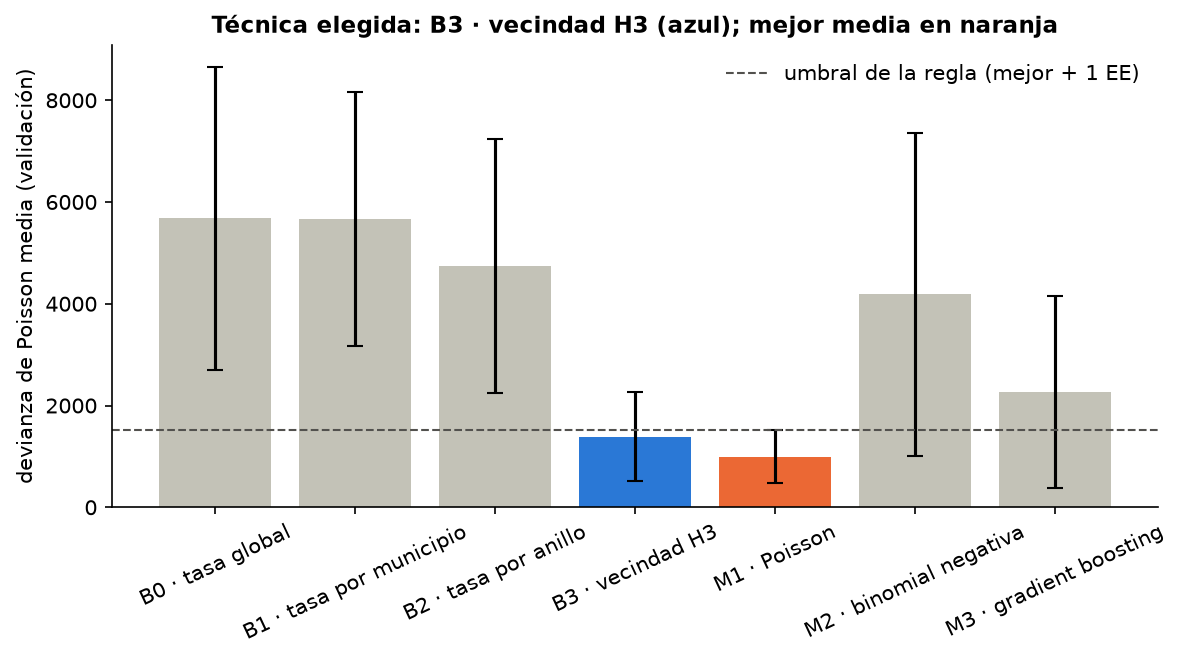
\includegraphics[width=0.72\textwidth]{imagenes/07_desarrollo/7_4_modelado/comparacion_tecnicas.png}
  \fuente{Elaboración propia, a partir de \var{04_modelado} (sección 6). Barras de error:
  $\pm 1$ error estándar; línea discontinua: umbral de la regla (mejor media más un error
  estándar); azul: técnica elegida; naranja: menor devianza media.}
\end{figure}

La tabla y la figura~\ref{fig:comparacion-tecnicas} permiten cinco lecturas:
\begin{enumerate}
  \item \textbf{Las líneas base por grupo apenas mejoran a la tasa global.} B1 y B2 tienen
        devianzas similares a B0, y su $D^2$ medio es negativo. En promedio predicen peor
        que la media del propio pliegue: una tasa común a todo un municipio o anillo no
        distingue entre zonas vecinas con comportamientos muy distintos.
  \item \textbf{La vecindad produce el mayor salto de la escalera.} B3 reduce la devianza
        de 4.743 a 1.389 y lleva el $D^2$ a 0,73. La información local es mucho más útil
        que las agrupaciones administrativas o por distancia.
  \item \textbf{M1 obtiene la menor devianza media (994,6)}, con un $D^2$ igual al de B3.
        Sin embargo, su calibración es de 0,807: en conjunto subestima el total de
        consultas en torno a un 19~\%.
  \item \textbf{M2 y M3 no compensan su complejidad.} M2 ordena bien las zonas (Spearman de
        0,843), pero su calibración de 0,354 indica que estima apenas un tercio del volumen
        real. Al corregir la sobredispersión da menos peso a las zonas de conteo alto,
        precisamente donde está casi todo el volumen. M3 alcanza un buen $D^2$ medio, pero
        su devianza es muy inestable entre pliegues.
  \item \textbf{La variabilidad entre pliegues es alta.} Las desviaciones estándar son del
        mismo orden que las medias. La tabla~\ref{tab:cv-pliegues} muestra la causa.
\end{enumerate}

\begin{table}[H]
  \centering
  \caption{Devianza de Poisson por pliegue de validación}
  \label{tab:cv-pliegues}
  \interlineadoSimple
  \small
  \begin{tabular}{@{}lrrrrr@{}}
    \toprule
    \textbf{Técnica} & \textbf{Pliegue 0} & \textbf{Pliegue 1} & \textbf{Pliegue 2} & \textbf{Pliegue 3} & \textbf{Pliegue 4} \\
    \midrule
    B0 & 2.811,7 & 3.914,3 & 17.477,0 & 2.510,8 & 1.666,5 \\
    B1 & 2.100,2 & 7.009,3 & 14.898,9 & 2.319,5 & 1.998,9 \\
    B2 & 2.274,0 & 2.886,6 & 14.697,3 & 2.052,4 & 1.803,1 \\
    B3 & 155,7 & 1.491,2 & 4.722,5 & 128,3 & 448,7 \\
    M1 & 145,5 & 1.199,8 & 2.956,3 & 241,8 & 429,6 \\
    M2 & 322,1 & 3.376,8 & 16.663,5 & 271,0 & 316,9 \\
    M3 & 107,2 & 971,0 & 9.753,8 & 147,5 & 349,9 \\
    \bottomrule
  \end{tabular}
  \fuente{Elaboración propia, a partir de \var{resultados/04_modelado/cv_por_pliegue.csv}.}
\end{table}

El pliegue 2 contiene bloques del centro de la ciudad, con conteos de decenas de miles de
consultas por zona, y su devianza es varias veces mayor que la de los demás en todas las
técnicas. Es ahí donde M3 falla más (9.753,8), probablemente porque sus árboles no
extrapolan bien a zonas con valores de los predictores poco frecuentes en el
entrenamiento de ese pliegue. En los pliegues periféricos (0, 3 y 4), B3, M1 y M3 tienen
errores de magnitud parecida. Esta heterogeneidad es la razón por la que la selección no
puede basarse solo en la media: la diferencia entre dos técnicas debe juzgarse frente a
la incertidumbre de esa media.

\subsection{Regla de selección}
\label{sec:regla-seleccion}

La técnica final se elige con una regla escrita en el protocolo antes de ejecutar ningún
modelo, conocida como \textbf{regla de un error estándar}: \emph{se elige la técnica más
simple de la escalera cuya devianza media no supere la mejor devianza media más un error
estándar de esta.}

El \emph{error estándar} (EE) mide cuánto podría variar la devianza media si los pliegues
fueran otros. Se calcula como la desviación estándar entre pliegues dividida por la raíz
del número de pliegues: $\text{EE} = \text{DE} / \sqrt{5}$. Dos técnicas cuyas medias
difieren menos de un EE no pueden distinguirse con los datos disponibles. En ese caso, la
regla prefiere la más simple, porque tiene menos supuestos, es más fácil de explicar y es
menos propensa al sobreajuste. La tabla~\ref{tab:regla-seleccion} aplica la regla.

\begin{table}[H]
  \centering
  \caption{Aplicación de la regla de un error estándar}
  \label{tab:regla-seleccion}
  \interlineadoSimple
  \small
  \begin{tabular}{@{}lrrcc@{}}
    \toprule
    \textbf{Técnica} & \textbf{\celda{Devianza\\media}} & \textbf{EE} & \textbf{\celda{$\leq$ umbral\\(1.518,8)}} & \textbf{Resultado} \\
    \midrule
    B0 & 5.676,1 & 2.972,1 & no & --- \\
    B1 & 5.665,3 & 2.494,1 & no & --- \\
    B2 & 4.742,7 & 2.495,1 & no & --- \\
    \textbf{B3} & \textbf{1.389,3} & \textbf{869,4} & \textbf{sí} & \textbf{elegida} \\
    M1 & 994,6 & 524,3 & sí & mejor media \\
    M2 & 4.190,1 & 3.174,7 & no & --- \\
    M3 & 2.265,9 & 1.878,3 & no & --- \\
    \bottomrule
  \end{tabular}
  \fuente{Elaboración propia, a partir de \var{resultados/04_modelado/regla_seleccion.csv}.
  Umbral $= 994{,}6 + 1{,}0 \times 524{,}3 = 1.518{,}8$.}
\end{table}

La mejor devianza media es la de M1 (994,6), con un error estándar de 524,3, lo que fija el
umbral en 1.518,8. Solo dos técnicas quedan por debajo: M1 y B3 (1.389,3). Como B3 ocupa
una posición anterior en la escalera, la regla \textbf{elige B3, el suavizado por vecindad
H3}.

La elección no responde a que B3 haya sido la primera técnica ejecutada ni a que tenga el
menor error. Las siete técnicas se evaluaron en las mismas condiciones y M1 obtuvo una
media menor. Se elige B3 porque la regla declarada de antemano establece que una diferencia
de 395 unidades de devianza, inferior a un error estándar, no justifica un modelo
paramétrico con supuestos que los propios datos contradicen, como la varianza igual a la
media. Hay además dos indicios, que no forman parte de la regla, a favor de B3 en el uso
previsto:
\begin{itemize}
  \item su calibración fuera de pliegue es de 0,977, frente a 0,807 de M1, de modo que
        reproduce mejor el volumen total;
  \item ordena las zonas algo mejor: calculado sobre todas las predicciones fuera de pliegue
        juntas, el Spearman es de 0,802 frente a 0,760. Estas cifras difieren de las de la
        tabla~\ref{tab:cv-resumen} (0,799 y 0,772), que son la media de los cinco valores
        calculados pliegue a pliegue.
\end{itemize}

La figura~\ref{fig:calibracion-oof} compara las predicciones fuera de pliegue de ambas
técnicas con lo observado.

\begin{figure}[H]
  \centering
  \caption{Observado frente a esperado fuera de pliegue: B3 y M1}
  \label{fig:calibracion-oof}
  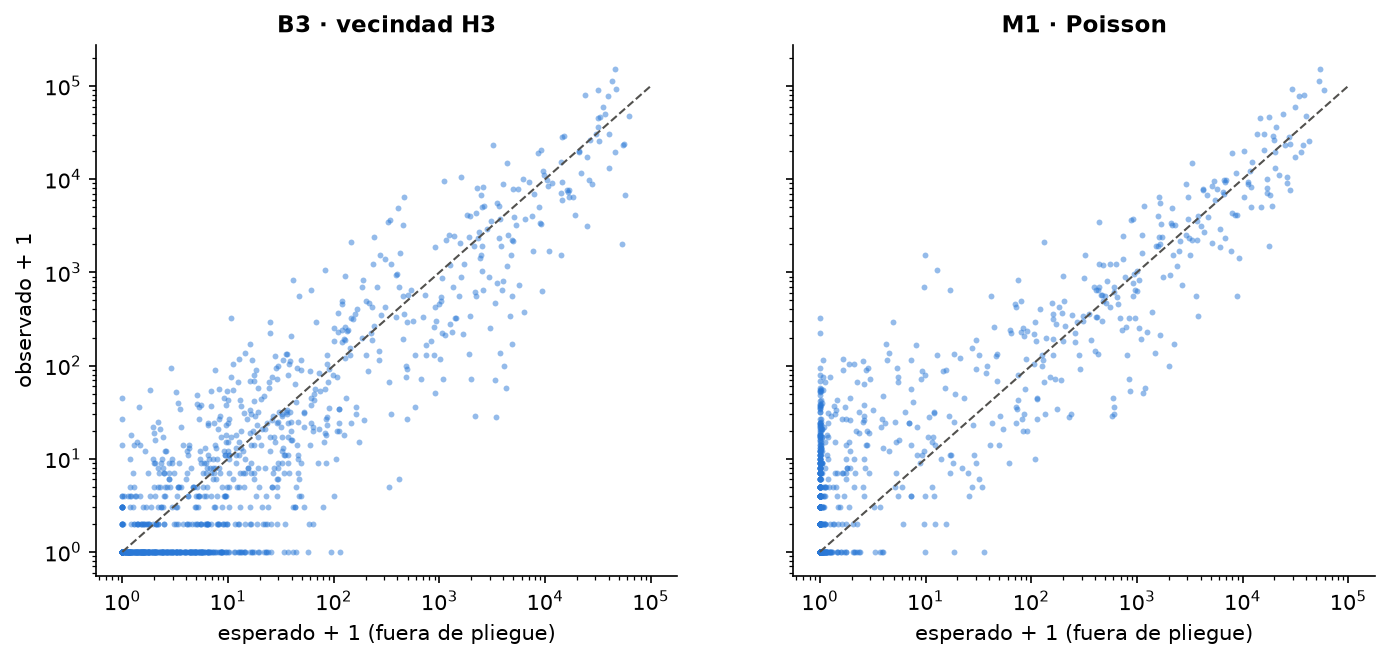
\includegraphics[width=0.9\textwidth]{imagenes/07_desarrollo/7_4_modelado/calibracion_oof.png}
  \fuente{Elaboración propia, a partir de \var{04_modelado} (sección 6). Ambos ejes en
  escala logarítmica (valor $+1$); la diagonal marca la coincidencia exacta.}
\end{figure}

Las dos nubes siguen la diagonal en los conteos altos, pero difieren en los bajos. B3
asigna a las zonas sin consultas esperados pequeños y variados, tomados de sus vecinas. M1
acumula muchas zonas con esperado cercano a cero, que en la columna izquierda aparecen con
conteos observados de hasta cientos de consultas. Esa diferencia es relevante para el
problema: una técnica que asigna esperado casi nulo a una zona no puede detectar en ella
una brecha negativa.

La técnica elegida tiene también un límite: B3 aprende de los vecinos, así que las zonas
que conviven con un polo de actividad heredan una tasa muy alta. Sus consecuencias se
examinan en la evaluación.
